
%(BEGIN_QUESTION)
% Copyright 2012, Tony R. Kuphaldt, released under the Creative Commons Attribution License (v 1.0)
% This means you may do almost anything with this work of mine, so long as you give me proper credit

The piston on a hydraulic ``bottle'' jack lifts up 1/8 of an inch for every stroke of the lever.  In each lever stroke, the handle end moves 14 inches.  Calculate the {\it mechanical advantage} of this hydraulic jack:

$$\includegraphics[width=15.5cm]{i02625x01.eps}$$

\underbar{file i02625}
%(END_QUESTION)





%(BEGIN_ANSWER)

The mechanical advantage of any machine may be empirically determined by dividing input displacement by output displacement:

$$M_A = {s_{in} \over s_{out}}$$

In this case, an input displacement of 14 inches yields an output displacement of 0.125 inches, so:

$$M_A = {14 \hbox{ in} \over 0.125 \hbox{ in}} = 112$$

This means the handle tip moves 112 times farther than the jack's lifting piston, but the lifting piston exerts 112 times more force than it takes to move the handle.

%(END_ANSWER)





%(BEGIN_NOTES)


%INDEX% Machine, hydraulic ``bottle'' jack
%INDEX% Machine, mechanical advantage

%(END_NOTES)


